\chapter{Riconoscitori LR}

\subsubsection{Parsing LR vs Parsing LL}
Costruendo l'albero top-down, la debolezza dell'analisi LL si traduce in:
\begin{itemize}
    \item deve poter identificare la produzione giusta usando soltanto i \textit{primi k simboli della parte destra}
    \item LL(1) è l'unico caso interessante
    \item LL(2) è utile in casi particolari
\end{itemize}

L'analisi LR invece, costruisce l'albero \textbf{bottom-up}:
\begin{itemize}
    \item parte dalle foglie, aspettando di avere abbastanza informazione per decidere come interpretarle
    \item meno naturale ma superiore dal punto di vista teorico
    \item ogni grammatica LL(k) è anche LR(k)
\end{itemize}

Tuttavia l'analisi LR è complessa da progettare e già il caso LR(1) spesso ingestibile per le grammatiche dei tipici linguaggi.

Sono state sviluppate \textit{tecniche semplificate}:
\begin{itemize}
    \item \textbf{SLR}: Simple LR
    \item \textbf{LALR}: Look-Ahead LR
\end{itemize}

Si utilizzano comunque sempre strumenti \textit{automatici}.

\begin{figure}[H]
    \caption{Gerarchia LR}
    \centering
    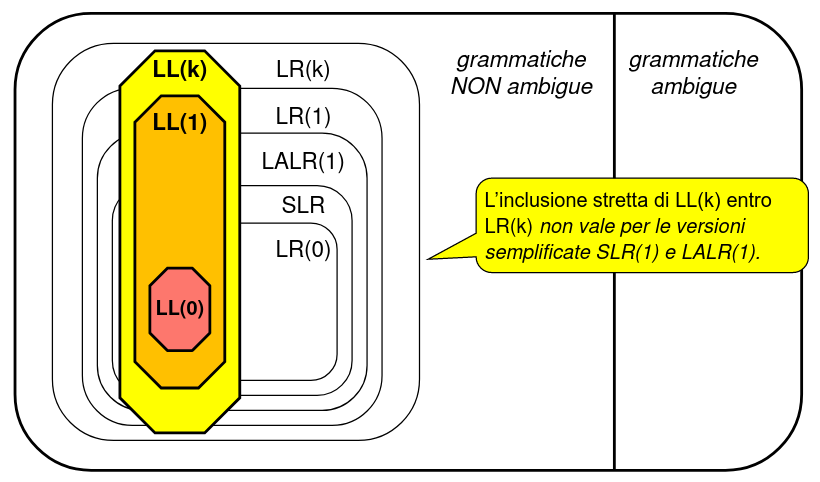
\includegraphics[width=0.7\textwidth]{/home/riccardoob/appunti/linguaggi/images/47.png}
\end{figure}

\subsubsection{Tecniche LR}
L'analisi LR procede BOTTOM UP, parte dalla frase e cerca di \textbf{riduarla} allo scopo S, ogni passo deve decidere se:
\begin{itemize}
    \item proseguire la lettura da input $\rightarrow$ \textbf{SHIFT}
    \item costruire un pezzo di albero $\rightarrow$ \textbf{REDUCE}
\end{itemize}

L'ultima REDUCE conclude l'albero con successo, accetta la frase nella fase di \textbf{ACCEPT}.

Per questo ha sempre bisogno di \textit{informazioni di contesto}.

\section{Architettura}
Il parser LR richiede un componenente, detto \textbf{ORACOLO}, che in base al contesto corrente, comunich se effettuare SHIFT o REDUCE al parser.

Un parser LR è quindi composto da:
\begin{itemize}
    \item un \textbf{oracolo}, che comunica se fare SHIFT o REDUCE
    \item uno \textbf{stack}, in cui conservare lo stato corrente di input e albero
    \item un \textbf{controller} che governa i primi due
\end{itemize}

\subsubsection{Informazione di contesto}
L'oracolo sfrutta opportune \textit{informazioni di contesto} per decidere se effettuare la lettura di un nuovo input o un passo di riduzione.

Questo componenente è un \textit{riconoscitore di contesti}, e solo se riconosce un appropriato \textit{contesto di riduzione}, ordina l'azione REDUCE appropriata per costruire senza ambiguità un certo pezzo di albero.

\section{Caso L(0)}

Nell'analisi LR conviene studiare per prima LR(0), un sottoinsieme di LR nel quale è possibile scegliere la mossa da fare \textit{senza dover guardare il prossimo simbolo di input}.

In LR questo non significa non avere informazioni in assoluto, si precludono quelle future ma si ritengono informazioni sul contesto passato.

\subsection{Analisi LR(0)}
Passi:
\begin{itemize}
    \item calcolare il \textit{contesto} LR(0) di ciascuna produzione
    \item identificare \textbf{collisioni} in contesti di produzioni diverse
    \begin{itemize}
        \item \textbf{collisione}: stringa appartenente a un contesto è un \textbf{prefisso proprio} di una stringa in un altro contesto
        \item \textbf{prefisso proprio}: una stringa è prefisso di un'altra e ciò che segue è un terminale (non metasimbolo)
    \end{itemize}
    \item se non ci sono collisioni, si possono usare i contesti LR(0) per guidare l'analisi
\end{itemize}

Se sono presenti collisioni, i contesti LR(0) non sono sufficienti, è necessario testare con LR(1).
\subsubsection{Esempio 1}
Grammatica LR(0):
\setlist{nosep}
\begin{multicols}{2}
    \begin{itemize}
        \item \texttt{S} $\rightarrow$ \texttt{a A b}
        \item \texttt{S} $\rightarrow$ \texttt{a a B b a}
        \item \texttt{A} $\rightarrow$ \texttt{A a}
        \item \texttt{A} $\rightarrow$ \texttt{b}
        \item \texttt{B} $\rightarrow$ $\varepsilon$
    \end{itemize}
    \columnbreak
    \begin{itemize}
        \item[] contesto LR(0): \texttt{\{aAb\}}
        \item[] contesto LR(0): \texttt{\{aaBba\}}
        \item[] contesto LR(0): \texttt{\{aAa\}}
        \item[] contesto LR(0): \texttt{\{ab\}}
        \item[] contesto LR(0): \texttt{\{aa\}}
    \end{itemize}
\end{multicols}
\setlist{}

Da notare che non esiste collisione tra i contesti \texttt{aaBba} e \texttt{aa}, perché la stringa \texttt{aa}, pur essendo un prefisso di \texttt{aaBba} non è \textit{prefisso proprio} di quest'ultima (\texttt{B} è un non terminale).

La frase \texttt{abab} è analizzata come segue:

\begin{figure}[H]
    \centering
    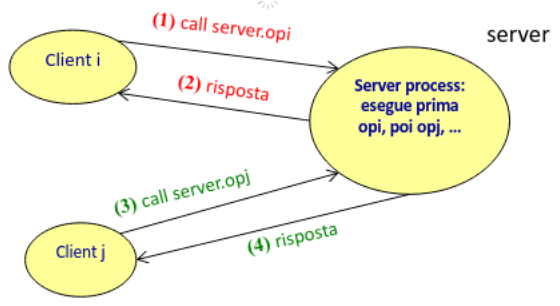
\includegraphics[width=\textwidth]{/home/riccardoob/appunti/linguaggi/images/48.png}
\end{figure}

Per ovviare a un possibile caso critico, conviene assumere che esista una produzione di \textbf{top-level} \texttt{Z} $\rightarrow$ \texttt{S}, dove \texttt{Z} è il nuovo scopo.

\subsubsection{Esempio 2}

\setlist{nosep}
\begin{multicols}{2}
    \begin{itemize}
        \item \texttt{S} $\rightarrow$ \texttt{a A b}
        \item \texttt{S} $\rightarrow$ \texttt{a a B b a}
        \item \texttt{A} $\rightarrow$ \texttt{A a}
        \item \texttt{A} $\rightarrow$ \texttt{b}
        \item \texttt{B} $\rightarrow$ $\varepsilon$
    \end{itemize}
    \columnbreak
    \begin{itemize}
        \item[] contesto LR(0): \texttt{\{aAb\}}
        \item[] contesto LR(0): \texttt{\{aaBba\}}
        \item[] contesto LR(0): \texttt{\{aAa\}}
        \item[] contesto LR(0): \texttt{\{ab\}}
        \item[] contesto LR(0): \texttt{\{aa\}}
    \end{itemize}
\end{multicols}
\setlist{}

La frase aaba è analizzata come segue:
\begin{figure}[H]
    \centering
    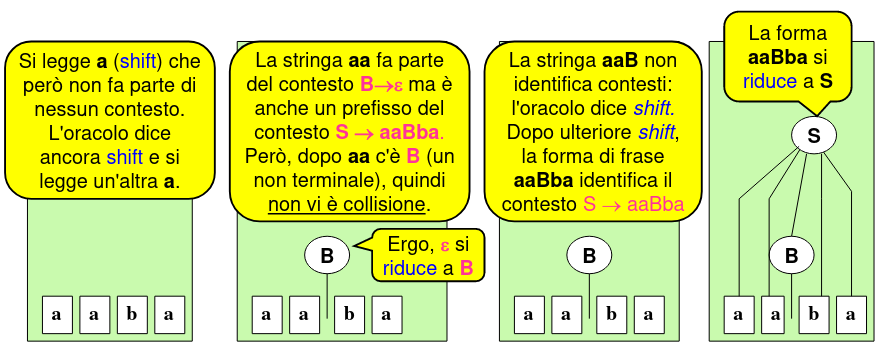
\includegraphics[width=\textwidth]{/home/riccardoob/appunti/linguaggi/images/49.png}
\end{figure}

L'emulatore richiede che la grammatica sia estesa con la regola top-level \texttt{Z} $\rightarrow$ \texttt{S}.
































